\documentclass[compress]{beamer}
\usetheme{Warsaw}
\usecolortheme{crane}
\usepackage[utf8]{inputenc}
\usepackage[portuguese]{babel}
\usepackage{url}
\usepackage{tikz}
\usepackage{color}
\usetikzlibrary{arrows}
\usetikzlibrary{arrows}
\usepackage{default}
\usepackage{amsmath}
\usepackage{amsfonts}
\usepackage{amssymb}
\usepackage{newalg}

% Algumas definições %%%
\def\term#1{{\sc #1}}   % IR terms in examples not index terms!
\def\query#1{{\sf #1}}
\def\oper#1{{\sc #1}} % AND, OR, NOT
%%%%%%%%%%%%%%%%%%%%%%%%

\title[Coelho: Dicionários e Recuperação Tolerante]
{Introdução à Recuperação de Informações\\
\large \url{https://github.com/fccoelho/curso-IRI}\\[0.5cm]
IRI 3: Dicionários e Recuperação Tolerante}

\author [Coelho F.C. \& Souza R.R.]{ Flávio Codeço Coelho}

\institute [EMAp, FGV]{Escola de Matemática Aplicada,   Fundação Getúlio Vargas}
\date


\begin{document}

\begin{frame}
\titlepage
\end{frame}

\begin{frame} %%%%%%%%%%%%%%%%%%%%%%%%%%%%%%
\frametitle{Sumário}
  \tableofcontents
\end{frame}

\section{Recapitulação}

\begin{frame}
\frametitle{Distinguindo entre Tipo e token}
\begin{itemize}
\item {\color{blue}Token} -- Uma instância de uma palavra ou termo ocorrendo 
em um documento
\item {\color{blue}Tipo} -- Uma classe de equivalência de tokens
\item \emph{In June, the dog likes to chase the cat in the barn.}
\item 12 tokens, 9 tipos de palavras
\end{itemize}
% $$L(x) = 1\cdot\frac{x - 2} {1 - 2}\cdot{\frac{x - 3}{1 - 3}}+{4}\cdot{\frac{x 
% - 1}{2 - 1}}\cdot{{x - 3}{2 - 3}}+{9}\cdot{\frac{x - 1}{3 - 1}}\cdot{\frac{x - 
% 2}{3 - 2}}$$
\end{frame}

\begin{frame}
\frametitle{Problemas na tokenização}
\begin{itemize}
\item Quais são os delimitadores? Espaços? Apóstrofes? 
Hífen? 
\item Para cada um destes: às vezes eles delimitam, às vezes não.
\item Muitas línguas não possuem espaços! (P.ex.,
Chinês)
\item Não Há espaços em palavras compostas em Holandês, Alemão e Sueco
(\emph{Lebensversicherungsgesellschaftsangestellter})
\end{itemize}
\end{frame}


\begin{frame}
\frametitle{Problemas com classes de equivalência}
\begin{itemize}
\item Um termo é uma classe de equivalência de tokens.
\item Como definir Classes de equivalência?
\item Números: (3/20/91 vs.\ 20/3/91)
\item Capitalização
\item Truncagem, Truncador de Porter 
\item Análise Morfológica : infleccional vs.\ derivacional
\item Problemas de classes de equivalências em outras línguas
\begin{itemize}
\item Morfologias mais complexas do que o inglês
\item Finlandês: Um único verbo pode ter 12000 formas diferentes
\item Acentos, tremas, etc.
\end{itemize}
\end{itemize}
\end{frame}

\begin{frame}[label=takeaway]
%\begin{frame}
\frametitle{Principais conclusões de hoje}

\begin{itemize}

\pause[2]

\item \myblue{Recuperação Tolerante:} O que fazer se não há correspondência 
exata entre o termo de consulta e os termos do documento.

\pause[3]

\item Consultas coringas

\pause[4]

\item Correção ortográficas

\end{itemize}

\end{frame}

\section{Dicionários}

\begin{frame}
\frametitle{Índice invertido}

Para cada termo $t$, armazenamos uma lista de documentos que contém $t$.

\bigskip

\begin{tabular}{|c|c|r|r|r|r|r|r|r|r|r|}
\cline{1-1}\cline{3-10}
\term{Brutus} & $\longrightarrow$ & 1 & 2 & 4 & 11 & 31 & 45 & 173 & 174 \\ 
\cline{1-1}\cline{3-10}
\multicolumn{8}{l}{} \\ \cline{1-1}\cline{3-11}
\term{Caesar} & $\longrightarrow$ & 1 & 2 & 4 & 5 & 6 & 16 & 57 & 132 & \ldots 
\\ \cline{1-1}\cline{3-11}
\multicolumn{8}{l}{} \\ \cline{1-1}\cline{3-6}
\term{Calpurnia} & $\longrightarrow$ & 2 & 31 & 54 & 101 \\
\cline{1-1}\cline{3-6} \multicolumn{8}{l}{}  \\
% The multicolumn{1}'s below suppress the vertical lines....
\multicolumn{1}{c}{$\vdots$} \\
\multicolumn{1}{c}{$\underbrace{\phantom{\mbox{Calpurnia}}}$} &
\multicolumn{1}{c}{} &
\multicolumn{9}{c}{$\underbrace{\phantom{\mbox{Calpurnia Calpurnia
Calpurnia Caesar hath}}}$} \\
\multicolumn{1}{c}{\alert<2>{\textbf{dicionário}}} &
\multicolumn{1}{c}{} & \multicolumn{9}{c}{\visible<1->{\textbf{postings}}}
\end{tabular}

\end{frame}

\begin{frame}
\frametitle{Dicionários}
\begin{itemize}[<+->]
\item O dicionário é a estrutura de dados que é usada para armazenar o 
vocabulário de termos.
\item {\color{blue}vocabulário de termos}: os {\color{blue}dados}
\item {\color{blue}Dicionário}: A {\color{blue} estrutura de dados} para 
armazenamento do vocabulário
\end{itemize}
\end{frame}

\begin{frame}
\frametitle{Dicionário como uma matriz com entradas de tamanho fixo}
\begin{itemize}[<+->]
\item Para cada termo, precisamos armazenar um par de ítens:
\begin{itemize}[<+->]
\item Frequência de documentos
\item Ponteiro para a lista de postings
\item \ldots
\end{itemize}
\item Assuma por ora que podemos armazenar esta informação em uma entrada de 
tamanho fixo.
\item Assuma que armazenamos estas entradas em uma matriz.
\end{itemize}
\end{frame}

\begin{frame}
\frametitle{Dicionário como uma matriz com entradas de tamanho fixo}

\begin{tabular}{l|lp{2cm}p{2cm}|}\cline{2-4}
&termo & documento frequência & ponteiro para %&
lista de postings 

\\\cline{2-4}
&a &656.265  & $\longrightarrow$ \\
&aachen &65 & $\longrightarrow$ \\
&\ldots & \ldots & \ldots \\
&zulu & 221 & $\longrightarrow$ \\\cline{2-4}
\multicolumn{1}{c}{espaço necessário:}& 20 bytes & 4 bytes & 
\multicolumn{1}{l}{4 bytes}
\\
\end{tabular}

\bigskip

\mygreen{como acessamos um termo de consulta $q_i$ nesta matriz em tempo de 
consulta? Ou seja: Que estrutura de dados usamos para localizar a 
entrada (linha) na matriz onde $q_i$ está armazenado?}

\end{frame}

\begin{frame}
\frametitle{Estruturas de dados para acessar os termos}
\begin{itemize}[<+->]
\item Duas Classes principais de estruturas de dados: hashes e árvores
\item Alguns sistemas de RI usam hashes, outros usam árvores.
\item Critérios de escolha:
\begin{itemize}[<+->]
\item Existe um número fixo de termos ou ele crescerá indefinidamente?
\item Quais as frequências relativas com que as várias chaves serão 
acessadas?
\item Quantos termos teremos?
\end{itemize}
\end{itemize}
\end{frame}

\begin{frame}
\frametitle{Hashes}
\begin{itemize}[<+->]
\item Cada termo do vocabulário é ``hasheado'' para um inteiro.
\item Busca-se evitar colisões
\item No momento da consulta, faz-se o seguinte: Hasheia o termo de 
consulta, resolve as colisões, Localiza entrada em uma matriz de 
elementos com tamanho constante
\item Prós: Busca em um hash é mais rápida do que em uma árvore.
\begin{itemize}[<+->]
\item Tempo de consulta é constante.
\end{itemize}
\item Contras
\begin{itemize}[<+->]
\item Não há forma de encontrar pequenas variações (\emph{resume} vs.\
  \emph{r\'{e}sum\'{e}})
\item Não permite busca de prefixos (Todos os termos que começam com
\emph{automat})
\item é necessário ``rehashear'' tudo periodicamente se o vocabulário continua 
crescendo.
\end{itemize}
\end{itemize}
\end{frame}


\begin{frame}
\frametitle{Árvores}
\begin{itemize}[<+->]
\item Árvores resolvem o problema do prefixo (Encontrar todos os termos 
começando com \emph{automat}).
\item Árvore mais simples: árvore binária
\item Busca é ligeiramente mais lenta que em hashes: $O(\log M)$,
  onde $M$ é o tamanho do vocabulário.
\item $O(\log M)$ vale apenas para árvores {\color{blue} balanceadas}.
\item Rebalancear árvores binárias é caro.
\item {\color{blue} Arvores-B} resolvem o problema do balanceamento.
\item Definição de árvore-B: cada nó interno tem um número de filhos no 
intervalo $[a,b]$ onde $a,b$ são inteiros positivos
  apropriados , p.ex., $[2,4]$.
%\item Note that we need a standard ordering for characters
%  in order to be able to use trees.
%\begin{itemize}[<+->]
%\item Not as simple with Chinese characters as with an alphabet
%\end{itemize}
\end{itemize}
\end{frame}


\begin{frame}
\frametitle{Árvore Binária}
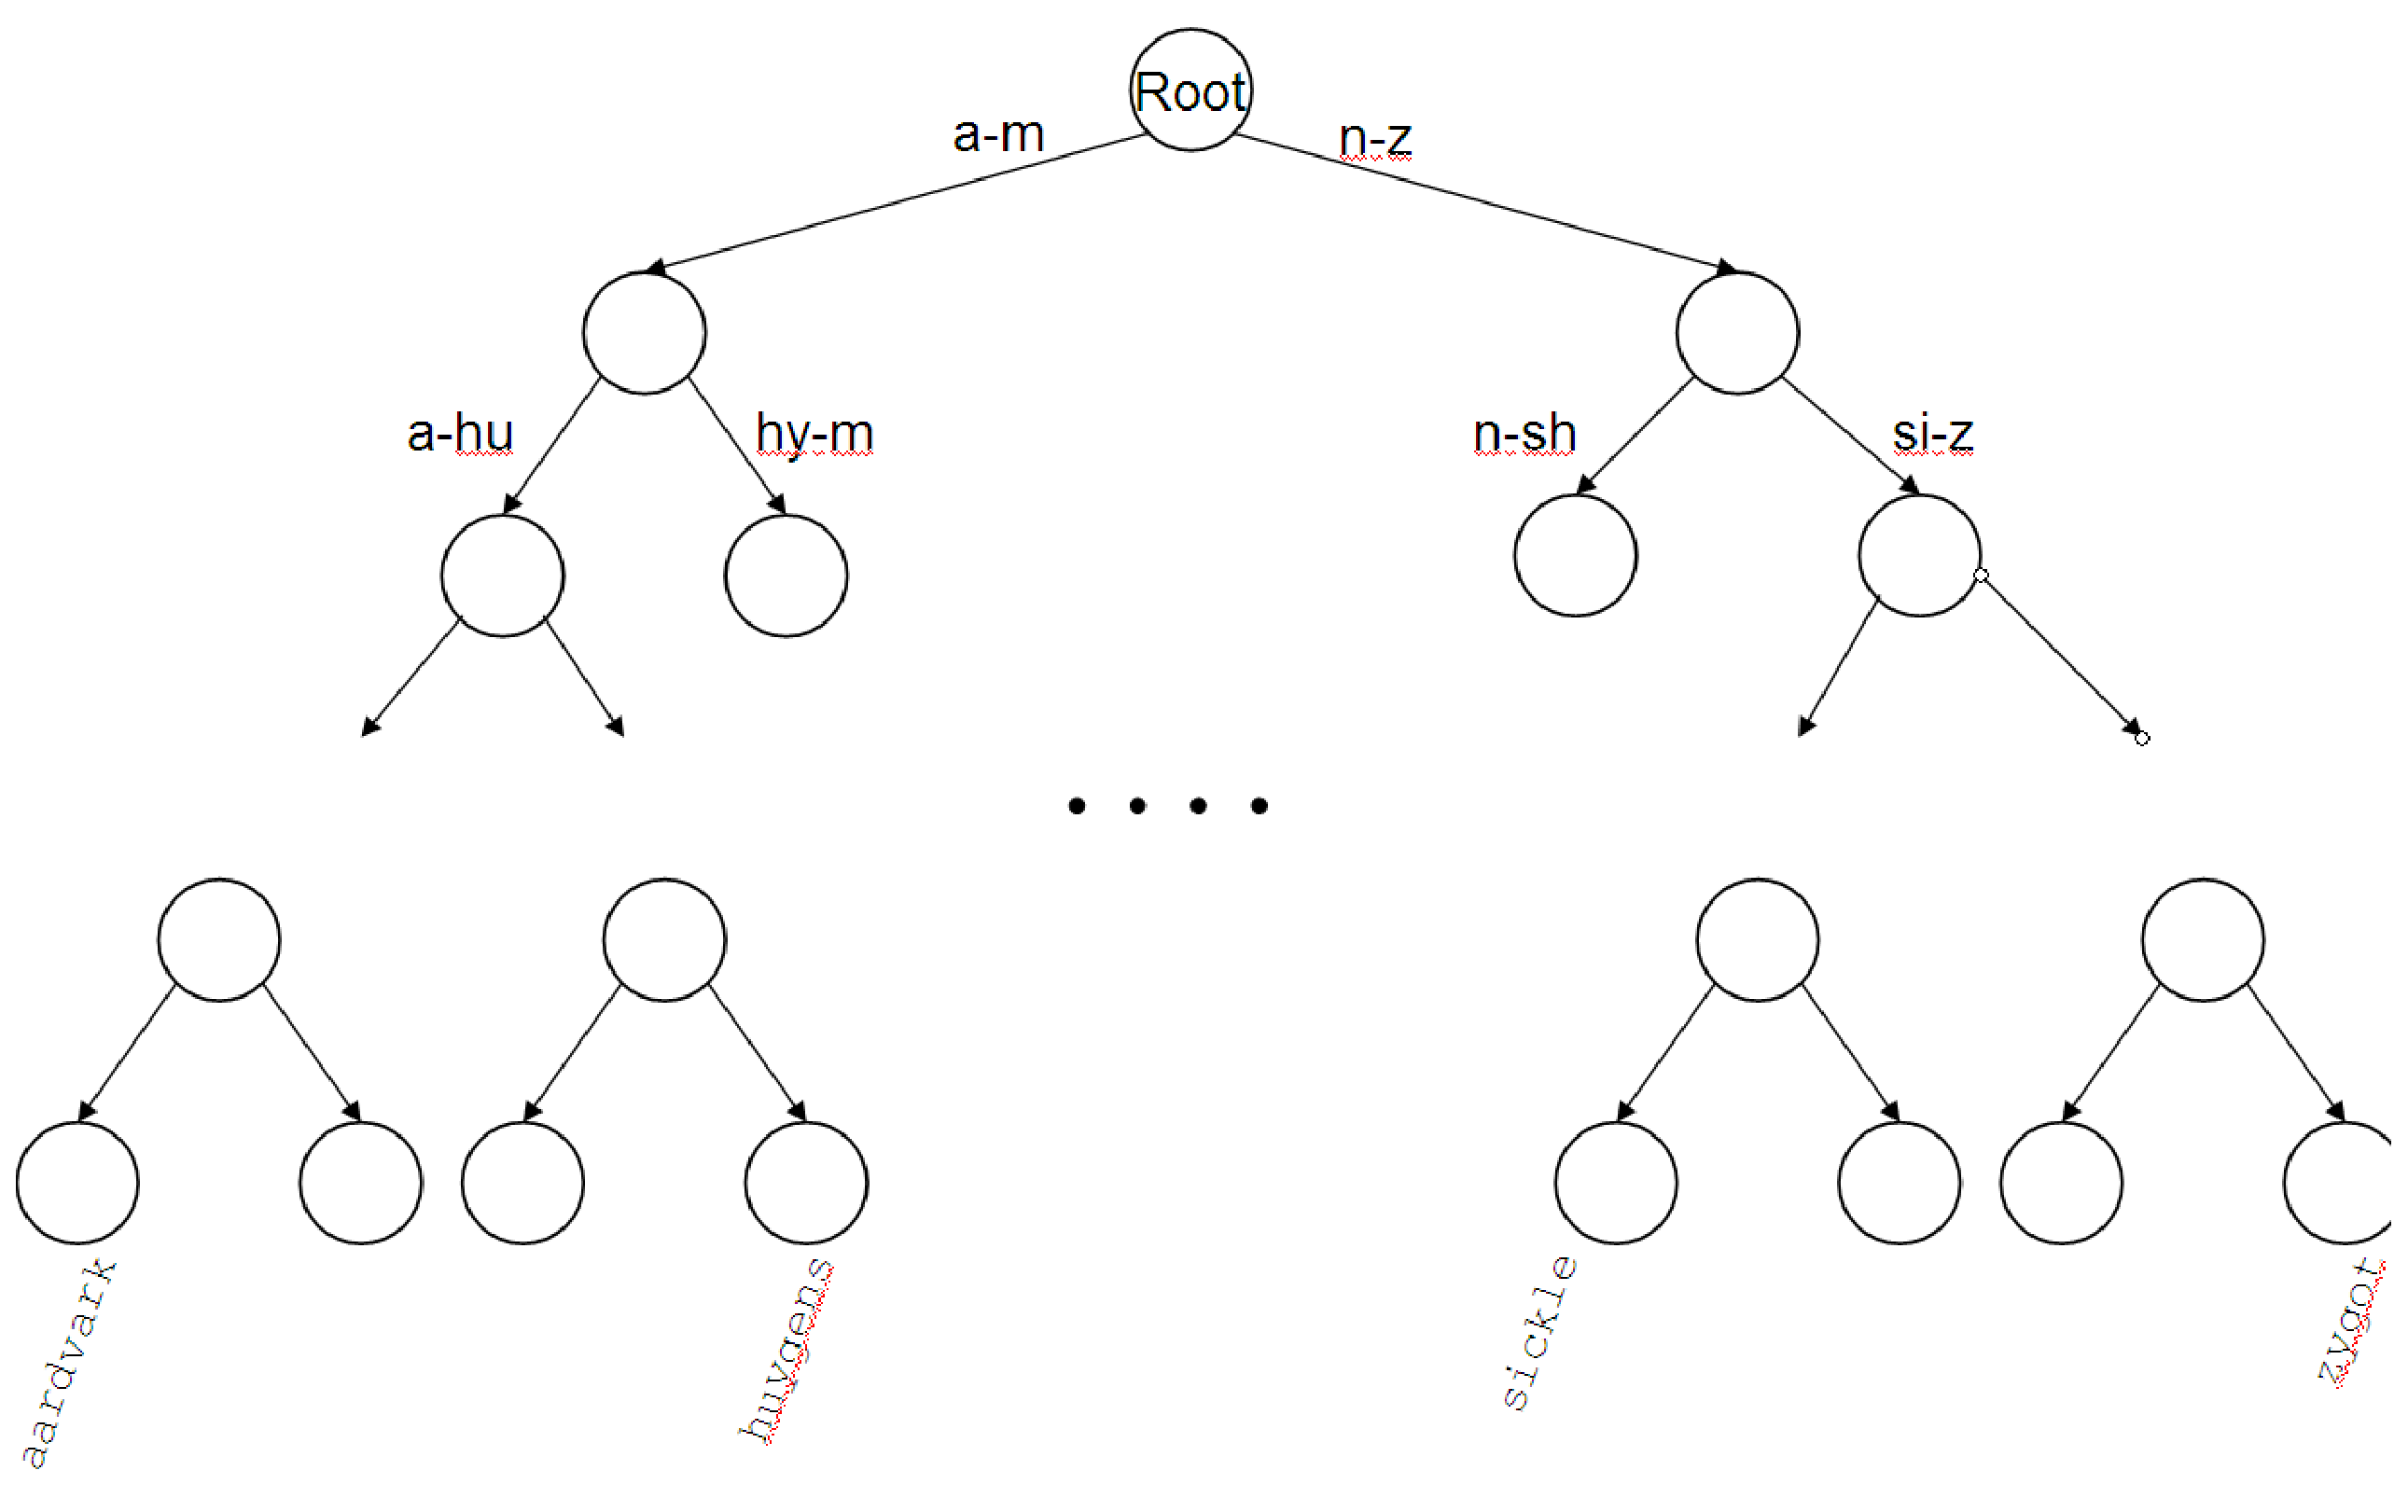
\includegraphics[width=11cm]{bst.eps}
\end{frame}

\begin{frame}
\frametitle{Árvore B}
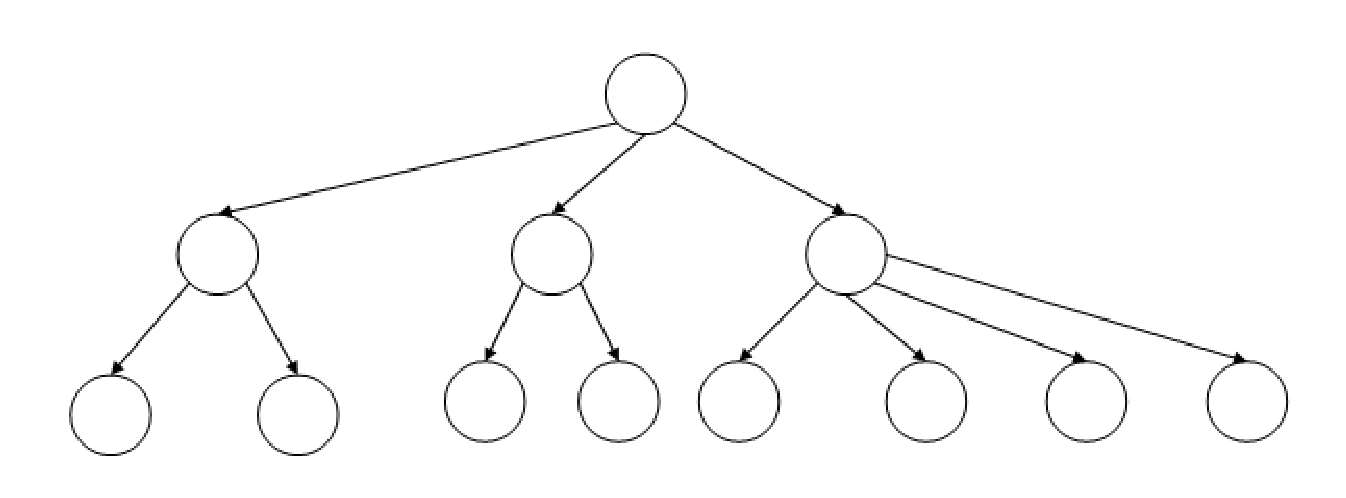
\includegraphics[width=11cm]{btree.eps}
\end{frame}
 
 \section{Consultas Coringa}

\begin{frame}
\frametitle{Consultas coringa}
\begin{itemize}[<+->]
\item \query{mon*}: Encontre todos os documentos contendo termos começados 
por \emph{mon}
\item Fácil com dicionários baseados em árvore B: recupera todos os termos $t$ 
no intervalo: $ \mbox{mon} \leq t < 
%%>
\mbox{moo}$
\item \query{*mon}: Encontre todos os documentos contendo termos que terminam 
com \emph{mon}
\begin{itemize}[<+->]
\item Mantém uma árvore adicional para termos  \emph{ao contrário}
\item Então recupera todos os termos $t$ no intervalo: $
  \mbox{nom} \leq t < 
%%>
\mbox{non}$
\end{itemize}
\item Resultado: Um conjunto de termos que correspondem à consulta 
coringa
\item Então recupera todos os documentos que contenham estes termos
\end{itemize}
\end{frame}

\begin{frame}
\frametitle{Como lidar com um * no meio de um termo}
\begin{itemize}[<+->]
\item Exemplo: \query{m*nchen}
\item Poderíamos buscar todos os termos que satisfazem \query{m*} e
\query{*nchen} Na árvore B e reter a interseção dos dois conjuntos.
\item Mas sai caro
\item Alternativa: índice {\color{blue} permuterm} 
\item Idéia básica: Rotaciona cada consulta coringa, de forma que o * ocorra no 
final.
\item Armazena cada uma destas rotações no dicionário, por exemplo, em uma 
árvore B
\end{itemize}
\end{frame}

\begin{frame}
\frametitle{Índice Permuterm }
\begin{itemize}[<+->]
\item Para o termo \term{hello}: adicione 
\emph{hello\$},
\emph{ello\$h},
\emph{llo\$he},
\emph{lo\$hel}, 
\emph{o\$hell}, e
\emph{\$hello}
  à árvore B onde \$ é um símbolo especial
\end{itemize}
\end{frame}

\begin{frame}
\frametitle{Permuterm $\rightarrow$ mapeamento de termos}
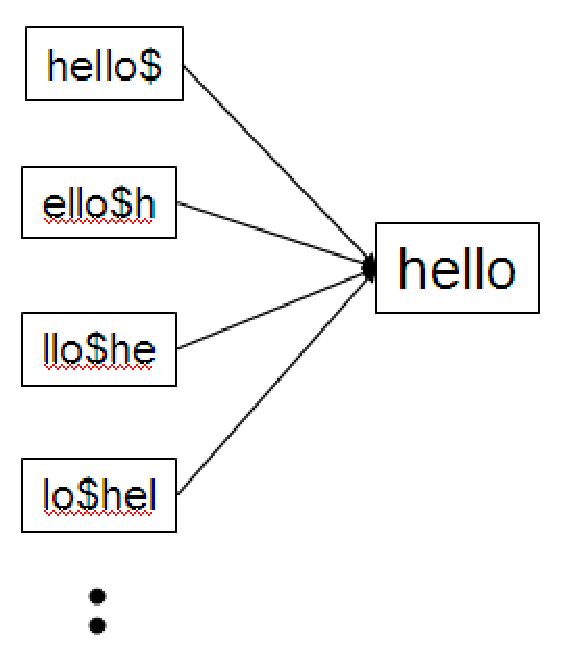
\includegraphics[width=5.5cm]{permuterm.eps}
\end{frame}

\begin{frame}
\frametitle{Permuterm index}
\begin{itemize}[<+->]
\item For \term{hello}, we've stored:
\emph{hello\$},
\emph{ello\$h},
\emph{llo\$he},
\emph{lo\$hel}, and
\emph{o\$hell}
\item Queries
\begin{itemize}[<+->]
\item For X, look up X\$
\item For X*, look up \$X*
\item For *X, look up X\$*
\item For *X*, look up X*
\item For X*Y, look up Y\$X*
\item Example: For hel*o, look up o\$hel*
%\item \mygreen{How do we handle X*Y*Z?}
\end{itemize}
\item Permuterm index would better be called a permuterm \myblue{tree}.
\item But permuterm index is the more common name.
\end{itemize}
\end{frame}

\begin{frame}
\frametitle{Processing a lookup in the permuterm index}
\begin{itemize}[<+->]
\item Rotate query wildcard to the right
\item Use B-tree lookup as before
\item Problem: Permuterm more than \myblue{quadruples} the size of the
  dictionary compared to a regular B-tree. (empirical number)
\end{itemize}
\end{frame}

\end{document}
